%%% Uncomment for presentation mode
\documentclass[10pt]{beamer}

%%% Uncomment for article mode
%\documentclass{article} 
%\usepackage{beamerarticle} 


\mode<presentation>
{
  \usetheme[]{Madrid}
  \useinnertheme{circles}
  \setbeamercovered{transparent=5}
  \setbeamertemplate{navigation symbols}{}
  \setbeamertemplate{frametitle continuation}[from second][\insertcontinuationtext]
}

\usepackage[english]{babel}
\usepackage[latin1]{inputenc}
\usepackage{times}
\usepackage[T1]{fontenc}
\usepackage{pgf,pgfplots}
\usepackage{color}
\usepackage{latexsym}
\usepackage[boxed,linesnumbered]{algorithm2e}
\usepackage{graphicx}
\usepackage{colortbl}
\usepackage[amssymb,thinspace]{SIunits}

\usepackage{tikz}
\usetikzlibrary{arrows,decorations,backgrounds,matrix,automata,trees,shapes,shadows,plotmarks,calc,positioning,patterns,chains}
\pgfdeclarelayer{background}
\pgfdeclarelayer{foreground}
\pgfsetlayers{background,main,foreground}

\newcounter{finalframe}

%\AtBeginSection[]
%{
%  \setcounter{finalframe}{\value{framenumber}}
%  \begin{frame}<beamer>{Outline of the Thesis}
%	\setcounter{framenumber}{\value{finalframe}}
%    \tableofcontents[currentsection,hideallsubsections]
%  \end{frame}
%}

\renewcommand\example[1]{{\color{black!50!green}#1}}

\renewcommand{\baselinestretch}{1.05}
\parskip 1.33ex

%!TEX root = ../thesis.tex

\newcommand{\mathname}[1]{\operatorname{\textit{#1}}}
\newcommand{\superscript}[1]{\ensuremath{^{\textrm{#1}}}}
\newcommand{\subscript}[1]{\ensuremath{_{\textrm{#1}}}}

%%%%%%%%%%%%%%%%%%%%%%%%%%%%%%%%%%%%%%%%%%%%%%%%%%%%
% PERSONAL LaTex MACROS 
% Courtesy Sebastian Sardina, RMIT Melbourne.
%%%%%%%%%%%%%%%%%%%%%%%%%%%%%%%%%%%%%%%%%%%%%%%%%%%%

%%%%%%%%%%%%%%%%%%%%%%%%%%%%%%%%%%%%%%%%%%%%%%%%%%%%
% Font modes & definitions
%%%%%%%%%%%%%%%%%%%%%%%%%%%%%%%%%%%%%%%%%%%%%%%%%%%%

% conditional math environment
% \gdef\Math#1{\ifmmode #1 \else \mbox{$#1$}\fi}
\newcommand{\Math}[1]{\ensuremath{#1}}

\newcommand{\modesf}[1]{{\Math{\mathsf{#1}}}}
\newcommand{\modecal}[1]{{\Math{\mathcal{#1}}}}
\newcommand{\modeit}[1]{{\Math{\mathit{#1}}}}


\newcommand{\textmath}[1]{{\mbox{\textit{#1}}}}



%%%%%%%%%%%%%%%%%%%%%%%%%%%%%%%%%%%%%%%%%%%%%%%%%%%%
% Proper names
%%%%%%%%%%%%%%%%%%%%%%%%%%%%%%%%%%%%%%%%%%%%%%%%%%%%
\newcommand{\propername}[1]{\mbox{\small\textsf{#1}}}
\newcommand{\AgentO}{\propername{AGENT-0}}
\newcommand{\AgentSpeak}{\propername{AgentSpeak(L)}}
\newcommand{\AgentSpeakF}{\propername{AgentSpeak(F)}}
\newcommand{\ASHOP}{\propername{A-SHOP}}
\newcommand{\CANMINUS}{\propername{\CAN$^{\A}$}}
\newcommand{\CANMINUST}{\propernametiny{Can$^{\cal C}$}}
\newcommand{\CAN}{\propername{CAN}}
\newcommand{\CANT}{\propernametiny{Can}}
\newcommand{\CANPLAN}{\propername{CANPlan}}
\newcommand{\CANPLANT}{\propernametiny{CanPlan}}
\newcommand{\CANPLANII}{\propername{CanPlan2}}
\newcommand{\CANPLANOR}{\propername{Can(Plan)}}
\newcommand{\CANGOAL}{\propername{CanGoal}}
\newcommand{\ConGolog}{\propername{ConGolog}}
\newcommand{\CLAIM}{\propername{CLAIM}}
\newcommand{\dMARS}{\propername{dMARS}}
\newcommand{\DAPL}{\propername{2APL}}
\newcommand{\GOAL}{\propername{GOAL}}
\newcommand{\GOALBDI}{\propername{GOAL}}
\newcommand{\Golog}{\propername{Golog}}
\newcommand{\GORITE}{\propername{GORITE}}
\newcommand{\IndiGolog}{\propername{IndiGolog}}
\newcommand{\JACK}{\propername{JACK}}
\newcommand{\JACKTM}{\propername{Jack\texttrademark}}
\newcommand{\JADEX}{\propername{JADEX}}
\newcommand{\JAM}{\propername{JAM}}
\newcommand{\JASON}{\propername{Jason}}
\newcommand{\JSHOP}{\propername{JSHOP}}
\newcommand{\JSHOPII}{\propername{JSHOP2}}
\newcommand{\PDT}{\propername{PDT}}
\newcommand{\PLACA}{\propername{PLACA}}
\newcommand{\Prometheus}{\propername{Prometheus}}
\newcommand{\PRS}{\propername{PRS}}
\newcommand{\RAP}{\propername{Rap}}
\newcommand{\SHOP}{\propername{SHOP}}
\newcommand{\SHOPII}{\propername{SHOP2}}
\newcommand{\SPARK}{\propername{SPARK}}
\newcommand{\TAPL}{\propername{3APL}}
\newcommand{\weka}{\propername{weka}}


%%%%%%%%%%%%%%%%%%%%%%%%%%%%%%%%%%%%%%%%%%%%%%%%%%%%
% Calligraphic letters 
% -- Taken from Giuseppe De Giacomo 2006
%%%%%%%%%%%%%%%%%%%%%%%%%%%%%%%%%%%%%%%%%%%%%%%%%%%%
\newcommand{\A}{\modecal{A}} \newcommand{\B}{\modecal{B}}
\newcommand{\C}{\modecal{C}} \newcommand{\D}{\modecal{D}}
\newcommand{\E}{\modecal{E}} \newcommand{\F}{\modecal{F}}
\newcommand{\G}{\modecal{G}} \renewcommand{\H}{\modecal{H}}
\newcommand{\I}{\modecal{I}} \newcommand{\J}{\modecal{J}}
\newcommand{\K}{\modecal{K}} \renewcommand{\L}{\modecal{L}}
\newcommand{\M}{\modecal{M}} \newcommand{\N}{\modecal{N}}
\renewcommand{\O}{\modecal{O}} \renewcommand{\P}{\modecal{P}}
\renewcommand{\S}{\modecal{S}} \newcommand{\T}{\modecal{T}}
\newcommand{\U}{\modecal{U}} \newcommand{\V}{\modecal{V}}
\newcommand{\W}{\modecal{W}} \newcommand{\X}{\modecal{X}}
\newcommand{\Y}{\modecal{Y}} \newcommand{\Z}{\modecal{Z}}
\newcommand{\R}{\modecal{R}} 


%%%%%%%%%%%%%%%%%%%%%%%%%%%%%%%%%%%%%%%%%%%%%%%%%%%%
% Margin notes for comments  
%%%%%%%%%%%%%%%%%%%%%%%%%%%%%%%%%%%%%%%%%%%%%%%%%%%%
\setlength{\marginparwidth}{0.1in}
\let\oldmarginpar\marginpar
\renewcommand\marginpar[1]{\-\oldmarginpar[\raggedleft\footnotesize #1]%
{\raggedright\footnotesize #1}}

\setlength{\marginparwidth}{0.5in}
\newcommand{\notem}[1]{\marginpar{\scriptsize  \textbf{#1}}}
\newcommand{\notems}[1]{\notem{S: #1}}
\newcommand{\noteml}[1]{\notem{L: #1}}
\newcommand{\notemd}[1]{\notem{D: #1}}

\newcommand{\ncheck}{\notem{CHECK!}}
\newcommand{\GGG}{\notem{GGG}}
\newcommand{\SSS}{\notem{SSS}}
\newcommand{\LIN}{\notem{LP}}
\newcommand{\YVES}{\notem{YL}}




%%%%%%%%%%%%%%%%%%%%%%%%%%%%%%%%%%%%%%%%%%%%%%%%%%%%
% PhD boxed notes for the committee in Toronto 
% -- Taken from Ron Petrick 2004
% -- Modified
%%%%%%%%%%%%%%%%%%%%%%%%%%%%%%%%%%%%%%%%%%%%%%%%%%%%
% \usepackage{color}
\newcounter{countphdnote}
%\newcommand{\phdnote}[1]{\textbf{#1}}
\newcommand{\phdnote}[1]{
%\vskip 0.25in
\noindent
%\begin{center}
%\begin{tabular}{c}
		\fbox{
%		\fcolorbox{black}{white}{
%			\begin{minipage}{0.96\textwidth}
			#1\addtocounter{countphdnote}{1}%
%			\end{minipage}
			}
		\fcolorbox{black}{black}{\textcolor
		{white}{\textbf{\ Note \thecountphdnote\ }}}
%\end{tabular}
%\end{center}
%\vskip 0.25in
}



%%%%%%%%%%%%%%%%%%%%%%%%%%%%%%%%%%%%%%%%%%%%%%%%%%%%
% Tighter lists 
% -- Taken from Lin Padgham 2007
%%%%%%%%%%%%%%%%%%%%%%%%%%%%%%%%%%%%%%%%%%%%%%%%%%%%
\newcounter{bean}

\newenvironment{tightenumerate}{
                \begin{list}{
                  {\mbox {
                      \arabic{bean}.\/}}}{\usecounter{bean}
                      \setlength{\itemsep}{-1pt}\setlength{\topsep}{0pt}}}{
                \end{list}}

\newenvironment{tightitemize}{
                \begin{list}{$\bullet$}{
                    \setlength{\itemsep}{-1pt}}{\setlength{\topsep}{0pt}}}{
                \end{list}}
%\setlength{\itemsep}{0pt}}{\setlength{\topsep}{0pt}}}{

\renewenvironment{tightenumerate}{\begin{enumerate}}{\end{enumerate}}
\renewenvironment{tightitemize}{\begin{itemize}}{\end{itemize}}




%%%%%%%%%%%%%%%%%%%%%%%%%%%%%%%%%%%%%%%%%%%%%%%%%%%%
% General useful macros
%%%%%%%%%%%%%%%%%%%%%%%%%%%%%%%%%%%%%%%%%%%%%%%%%%%%

% Produces citations as follows: Author (Year)
\newcommand{\citeby}[1]{\citeauthor{#1} (\citeyear{#1})}

% Mark pages (pp. xxx)
\newcommand{\page}{pp.}

% Marker text
\newcommand{\marker}[1]{\textbf{******* \today: #1 *******}}

% Good underline --- Ttaken from Hector Levesque 2003
%	underline with space between text and line
\newcommand{\under}[1]{\mbox{\underline{\it\smash{#1}\vphantom{\lower.05ex\hbox{
x}}}}}

% \newcommand{\defterm}[1]{\under{\textit{#1}}}
\newcommand{\defterm}[1]{\textit{#1}}

% Comments -- just ignore everything: same as \comment{} in comment package
\newcommand{\commentarea}[1]{}

% Finish a page compactly (remove trailing space)
\newcommand{\finishpage}{ \newpage{ \pagestyle{empty} } }

% Separation for itemizations
\newcommand{\separation}[1]{\addtolength{\itemsep}{#1}}


% Italic text
\newcommand{\ii}[1]{\textit{#1}}

%%%%%%%%%%%%%%%%%%%%%%%%%%%%%%%%%%%%%%%%%%%%%%%%%%%%
% Thesis macros
%%%%%%%%%%%%%%%%%%%%%%%%%%%%%%%%%%%%%%%%%%%%%%%%%%%%

\newcommand{\subgoal}{sub-goal}


%%%%%%%%%%%%%%%%%%%%%%%%%%%%%%%%%%%%%%%%%%%%%%%%%%%%
% EOF: macros-sebastian.tex
%%%%%%%%%%%%%%%%%%%%%%%%%%%%%%%%%%%%%%%%%%%%%%%%%%%%

%Travelling Domain
\newcommand{\gTravel}{\propername{Travel}}
\newcommand{\pCycle}{\propername{Cycle}}
\newcommand{\pFly}{\propername{Fly}}
\newcommand{\pTram}{\propername{Tram}}
\newcommand{\pTrain}{\propername{Train}}
\newcommand{\pDest}{\propername{dist}}
\newcommand{\vCity}{\propername{long}}
\newcommand{\vWork}{\propername{short}}
\newcommand{\pWeather}{\propername{outlook}}
\newcommand{\vSunny}{\propername{sun}}
\newcommand{\vRaining}{\propername{rain}}
\newcommand{\pMoney}{\propername{money}}

%----------------------------------------------------------------------------
%----------------------------------------------------------------------------
\title[BDI Learning in Changing Environments]{Integrating Learning into a BDI Agent for Environments with Changing Dynamics}
\author[Singh et al.]{Dhirendra~Singh\inst{1} \and Sebastian~Sardina\inst{1} \and Lin~Padgham\inst{1} \and Geoff~James\inst{2}}
\institute[RMIT \& CSIRO]{
\inst{1}RMIT University, Melbourne, Australia \and 
\inst{2}CSIRO Energy Technology, Sydney, Australia
}
\date[IJCAI 2011]{International Joint Conference on Artificial Intelligence\\July 2011, Barcelona, Spain}
%----------------------------------------------------------------------------
%----------------------------------------------------------------------------


\begin{document}



%----------------------------------------------------------------------------
\begin{frame}[plain]
\setcounter{framenumber}{0}
\titlepage
\end{frame}


%----------------------------------------------------------------------------
%----------------------------------------------------------------------------
\section{Introduction}

%----------------------------------------------------------------------------
\begin{frame}[<+->]{Belief-Desire-Intention (BDI) Agent Architecture}
\action{}
\begin{center}
\resizebox{.75\paperwidth}{!}{
%!TEX root = ../dsingh-ijcai11-talk.tex
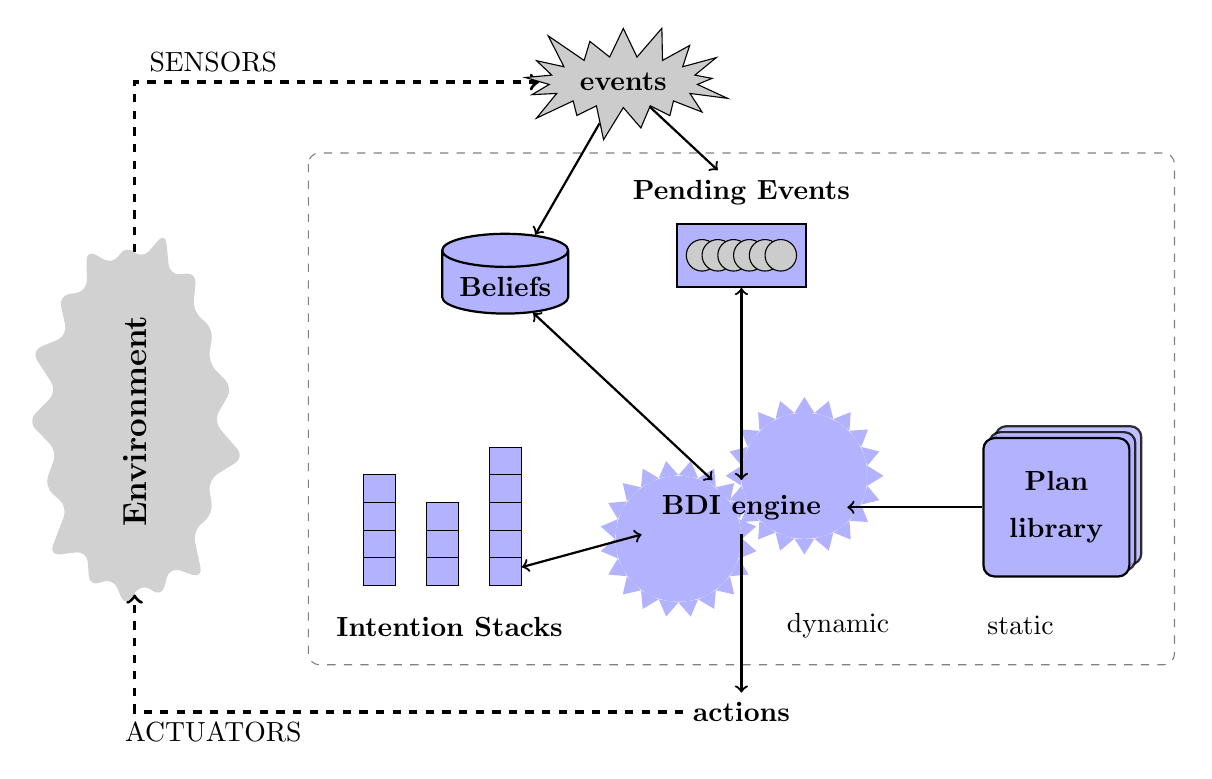
\begin{tikzpicture}

\tikzstyle{centityd}=[draw=black]
\tikzstyle{centityf}=[fill=blue!30]
\tikzstyle{centity}=[centityd,centityf]
\tikzstyle{entity}=[centity,thick,text centered,anchor=center]


\node[anchor=east] at (6,4.5)  {dynamic};
\node[anchor=west] at (7,4.5) {static};


\node (database) at (1,8.8)  (B)
	[cylinder,entity,shape border rotate=90,minimum width=1.6cm,shape aspect=.3]
	{\textbf{Beliefs}};


\node  (environment)  
       [below left of=B, rounded corners, minimum height=3cm,
       starburst,fill=black!18,rotate=90,shift={(-1cm,4cm)}] 
       {\textbf{\large Environment}};



\node at (4,10) (eventQueue) {{\bf Pending Events}};
\begin{pgfonlayer}{foreground}
\foreach \x in {3.5,3.7,...,4.5}
\draw [fill=black!20](\x,9.2) circle (0.2);
\end{pgfonlayer}
%\path (4,9.1) node (Q) {}; 
\draw (4,9.2) node (Q) 
	[entity, text width=1.4cm, minimum height=0.8cm] {};




\foreach \x in {4,3,2,1}
\draw (-.6,5) node (I) [anchor=south,draw, centity, text width=.5em,
	minimum height=\x em]{};
\foreach \x in {3,2,1}
\draw (0.2,5) node (I) [anchor=south,draw,centity, text width=.5em,
	minimum height=\x em]{};
\foreach \x in {5,4,3,2,1}
\draw (1,5) node (I) [anchor=south,draw, centity, text width=0.5em,
	minimum height=\x em]{};
\node[below left of=I] (Intentions) {{\bf  Intention Stacks}};


% { [start chain=1]
% % \node [on chain,draw] at (0,6) {};
%     \foreach \x in {1,2,...,11} {
%        \x, \node [draw,on chain=1] {};
%     }
% }

\begin{pgfonlayer}{foreground}
\node[anchor=center] at (4,6)  (deli) 
	{\begin{tabular}{c}
     	\textbf{BDI engine} 
     \end{tabular}};
\node at (4,3.4) (actions) {{\bf actions}};
\node at (2.5,11.4) [starburst,centityd,fill=black!20] (in) {{\bf events}};


\draw node (P) 
	[right of=deli,xshift=3cm,rounded corners, double copy
	shadow={opacity=0.8},text centered, entity, minimum height=5em] 
	{	\begin{tabular}{c} 
          \textbf{Plan} \\[1ex]
          \textbf{library}
         \end{tabular}	};



\draw[thick,->] (in) -- (B) ; 
\draw[thick,->] (in) -- (eventQueue) ; 
\draw[thick,->] (deli) -- (actions) ; 
\draw[thick,<->] (deli) -- (I) ; 
\draw[thick,<->] (deli) -- (B) ; 
\draw[thick,<-] (deli) -- (P) ;
\draw[thick,<->] (deli) -- (Q) ; 
\end{pgfonlayer}








\begin{pgfonlayer}{background}

%% Dotted box encapuslating the agent
\path (-1.5,10.5) node (c) {};
\path (9.5,4) node (d) {};
\path[fill=none,rounded corners, draw=black!50, dashed] (c) rectangle (d);




\draw[->,very thick,dashed] (environment) 
		|- node[above,xshift=1cm] {SENSORS}
	 	(in);
\draw[->,very thick,dashed] (actions.west) 
		-| node[below,xshift=1cm] {ACTUATORS}
		(environment.west);
\end{pgfonlayer}


\foreach \x in {-9,9,...,360}
\fill [rotate around={\x:(3.2,5.6)},centityf] 
	(4.0,5.4743) -- (4.2 ,5.6) -- (4.0,5.7257) -- (4.0,5.3487);
\fill [centityf] (3.2,5.6) circle (0.8);

\foreach \x in {0,18,...,360}
\fill [rotate around={\x:(4.8,6.4)},centityf] 
	(5.6,6.2743)-- (5.8,6.4) -- (5.6,6.5257) -- (5.6,6.2743);
\fill [centityf] (4.8,6.4) circle (0.8);


\end{tikzpicture}
}
\vskip 0.25cm
A \alert{plan} is a programmed recipe for achieving a goal in some situation.\\\action{We wish to \alert{improve plan selection} in situations, based on actual experience.}
\end{center}
\note{

-If I had to explain my thesis in one slide, then this is it. 

-Ignoring the details, all I want you to take from this slide is: that a BDI agent is programmed with a bag of tricks, or a library of plans, that it has to choose from in any given situation.

-What we would like is for the agent to learn what plans work best in which situations, based on ongoing experience.

-With this in mind, let's have a look at the outline of the talk.

BDI:
Influence of Rao \& Georgeff, Cohen and Levesque. 
The problem of plan selection.

BDI advantages:
1. Is robust and well suited for dynamic environments.
2. Has inspired several development platforms (PRS, AgentSpeak(L), JACK, JASON, SPARK, 3APL and others).
3. Has been deployed in practical systems like UAVs.

}

\end{frame}

%----------------------------------------------------------------------------
%----------------------------------------------------------------------------
%\begin{frame}[<+->]{Related Work in BDI Learning}
%
%\begin{block}{}\centering Little existing work in combining BDI reasoning with online learning\end{block}
%
%\begin{itemize}
%\item Existing work in BDI learning uses \alert{offline} learning, so {\em no learning takes place after deployment}.
%\item Learning in \alert{hierarchical task network (HTN) planning} is related but also is inherently offline.
%\item \alert{Hierarchical reinforcement learning} deals with similar issue to ours but is very different to agent programming.
%\end{itemize}
%
%\end{frame}


%----------------------------------------------------------------------------
%----------------------------------------------------------------------------
\section{A BDI Learning Framework}

%----------------------------------------------------------------------------
\begin{frame}{Plan Selection in a BDI Goal-Plan Hierarchy}
\begin{center}%!TEX root = ../aamas11storage.tex
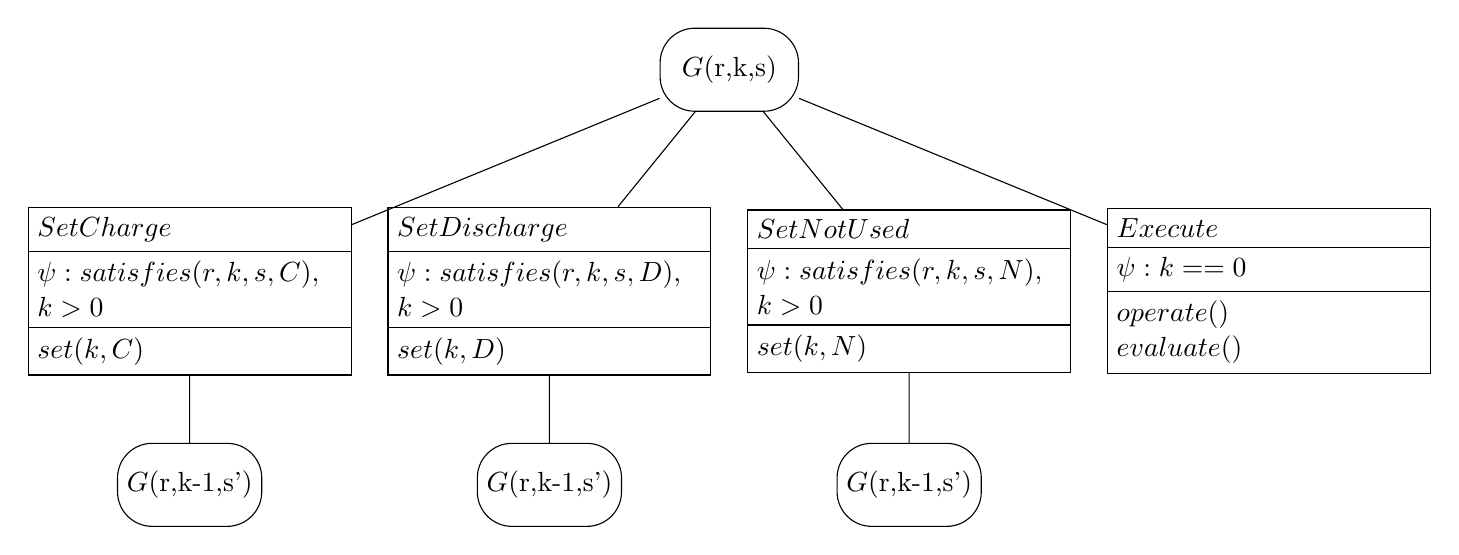
\begin{tikzpicture} [level distance=8.0em]
\tikzstyle{planbox}=[draw,text width=11.0em,rectangle split,rectangle split parts=3]
\tikzstyle{goalbox}=[draw,rounded corners=1.25em,minimum height=3em,minimum width=5em]

	
\tikzstyle{level 1}=[sibling distance=13.0em] 
\tikzstyle{level 2}=[level distance=7.0em] 

\node[goalbox,solid] {$G($r,k,s$)$}
	child {node[planbox] {$SetCharge$ 
			\nodepart{second} $\psi:satisfies(r,k,s,C),$\\$k>0$
			\nodepart{third} $set(k,C)$
		}
		child {node[goalbox] {$G($r,k-1,s'$)$}}
	}
	child {node[planbox] {$SetDischarge$ \nodepart{second}
			\nodepart{second} $\psi:satisfies(r,k,s,D),$\\$k>0$
			\nodepart{third} $set(k,D)$
		}
		child {node[goalbox] {$G($r,k-1,s'$)$}}
	}
	child {node[planbox] {$SetNotUsed$ \nodepart{second}
			\nodepart{second} $\psi:satisfies(r,k,s,N),$\\$k>0$
			\nodepart{third} $set(k,N)$
		}
		child {node[goalbox] {$G($r,k-1,s'$)$}}
	}
	child {node[planbox] {$Execute$ 
			\nodepart{second} $\psi:k==0$
			\nodepart{third} $operate()$ \\$evaluate()$
		}
	}
;

\end{tikzpicture}


\end{center}

\begin{center}
For plan $P_1$ to succeed, \alert{several correct choices must be made}.
\end{center}
\note{

The figure shows an example BDI plan library represented as a tree. Here plans nodes are suffixed with the label $P$ and goals with $G$. The parent of a plan is the goal type it was designed to handle. The children are sub-goals that must succeed in a sequential manner in order for the plan to succeed. Leaf plans interact directly with the environment by performing actions that may succeed (ticks) or fail (crosses) for a given world state. Here the successful resolution of the top-level goal requires 3 sequential actions to be performed.

What are we learning? The actual conditions under which a plan works once deployed. 

Why learn? For complex domains it may not be possible to accurately program all situations under which a plan is useful. Even so, the environment may change after the agent is deployed.

How do we do it? Add a machine learning filter over the programmed applicability conditions of plans, and learn this over time.

We're not learning a new plan or altering some existing plan. We're just learning when to use it.
}
\end{frame}

%----------------------------------------------------------------------------
\begin{frame}{The Learning Framework}

Augment \alert{a decision tree per plan}. \example{State representation includes world features, event parameters, and context variables.}
\vskip 1em

\begin{columns}
\begin{column}[l]{0.4\textwidth}
\begin{overlayarea}{\columnwidth}{5cm} 
\only<2->{
%!TEX root = ../dsingh-pgconf10.tex
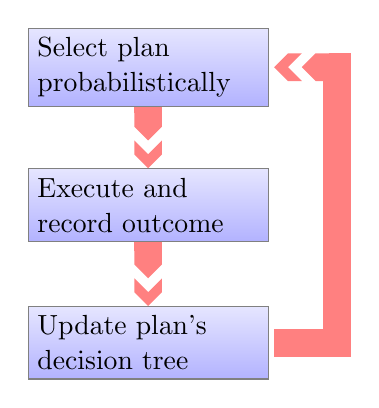
\begin{tikzpicture}
                    
\tikzstyle{box}=[text width=8em, draw=black!50, top color=blue!10, bottom color=blue!30]
\tikzstyle{pointer}=[color=red!50,->,>=fast cap,line width=10pt]

\node [box] at (0,0)  (A) {Select plan\\ probabilistically};
\node [box] at (0,-1.75) (B) {Execute and\\ record outcome};
\node [box] at (0,-3.5) (C) {Update plan's\\ decision tree};
\draw [pointer] (A) to [] (B); 
\draw [pointer] (B) to [] (C); 
\draw [pointer] (1.6,-3.5) -- (2.4,-3.5) -- (2.4,0) -- (1.6,0); 

\end{tikzpicture}

}
\end{overlayarea}
\end{column}
\begin{column}[l]{0.6\textwidth}
\begin{overlayarea}{\columnwidth}{5cm} 
\only<3-7>{
\begin{enumerate}
\item<3-7> For every plan whose programmed applicability condition holds, calculate a \alert{selection weight} based on perceived likelihood of success.
\item<4-7> \alert{Select} a plan probabilistically using selection weights.
\item<5-7> \alert{Execute} the plan (hierarchy) and record the outcome(s).
\item<6-7> \alert{Update} the plan's decision tree.
\item<7> Repeat.
\end{enumerate}
}
\only<8->{
\begin{columns}
\begin{column}[l]{0.15\textwidth}
\begin{tabular}{ c c }
$w_a$ & $\times$ \\
\alert{$w_b$} & \alert{$\times$} \\
$\ldots$ & \\
$\ldots$ & \\
\example{$w_b$} & \example{$\surd$} \\
$\ldots$ & \\
$\ldots$ & \\
$w_a$ & $\surd $ \\
$\ldots$ & \\
$\ldots$ & \\
\end{tabular}
\end{column}
\begin{column}[l]{0.85\textwidth}
\begin{itemize}
\item<9-> Incomplete data
\item<10-> Inconsistent data
\item<11-> Non-deterministic actions
\item<12-> Non-deterministic hierarchies
\item<13-> Dealing with failure recovery
\item<14-> Changing environment dynamics
\end{itemize}
\end{column}
\end{columns}
}
\end{overlayarea}
\end{column}
\end{columns}

\begin{overlayarea}{\columnwidth}{1cm} 
\only<15->{
\vskip -1em
\begin{block}{}\centering{Need a quantitative \alert{measure of confidence} in the current learning.}\end{block}
}
\end{overlayarea}

\note{
Touch on hierarchical learning issue, noisy training data, incomplete training data, non-deterministic domain, parameterised and recursive structures, confidence in learning, and now learning in environments with changing dynamics. Mention that we will expand on the final two.
}

\end{frame}

%----------------------------------------------------------------------------
%----------------------------------------------------------------------------
\section{Determining Confidence in Ongoing Learning}

%----------------------------------------------------------------------------
\begin{frame}{A Dynamic Confidence Measure}

\begin{columns}
\begin{column}[l]{0.4\textwidth}
\begin{overlayarea}{\textwidth}{5cm} 
\resizebox{\textwidth}{!}{
%!TEX root = ../dsingh-phdtalk.tex
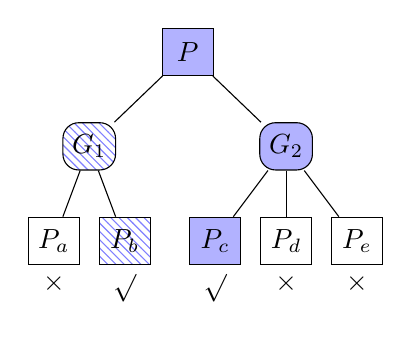
\begin{tikzpicture}[level distance=1.2cm]
\tikzstyle{succ}=[label=below:$\surd$]
\tikzstyle{fail}=[label=below:$\times$]
\tikzstyle{trace}=[solid,style=circle,fill=black!20,above left=0.15cm,scale=.7]

\tikzstyle{planbox}=[draw,minimum height=0.6cm,minimum width=0.65cm]
\tikzstyle{goalbox}=[draw,minimum height=0.6cm,minimum width=0.65cm,rounded corners=0.2cm]
\tikzstyle{planbox2}=[planbox,pattern=north west lines,pattern color=blue!50]
\tikzstyle{goalbox2}=[goalbox,pattern=north west lines,pattern color=blue!50]
\tikzstyle{goalbox3}=[goalbox,fill=blue!30]
\tikzstyle{planbox3}=[planbox,fill=blue!30]

\tikzstyle{level 1}=[sibling distance=2.5cm] 
\tikzstyle{level 2}=[sibling distance=0.9cm] 

\node[planbox3,solid] {$P$}
				child[solid] {node[goalbox2] {$G_{1}$}
					child {node[planbox,fail] {$P_{a}$}}
					child {node[planbox2,succ] {$P_{b}$}}
				}
				child[solid] {node[goalbox3] {$G_{2}$}
					child {node[planbox3,succ] {$P_{c}$}}
					child {node[planbox,fail] {$P_{d}$}}
					child {node[planbox,fail] {$P_{e}$}}
				}

;

\end{tikzpicture}

}
\end{overlayarea}
\end{column}
\begin{column}[l]{0.6\textwidth}
\begin{overlayarea}{\textwidth}{5cm} 
We build confidence from \alert{observed performance} of a plan using:
\pause
\begin{itemize}
\item<+-> \example{how well-informed were the recent decisions}, or \alert{stability-based} measure
\item<+-> \example{how well we know the worlds we are witnessing}, or \alert{world-based} measure
\item<+-> an averaging window $n$ and preference bias $\alpha$ \\~\\~\\
\end{itemize}
\end{overlayarea}
\end{column}
\end{columns}
\vskip -1cm
\uncover<5->{Plan selection weight, that dictates \alert{exploration}, is then calculated using the predicted \alert{likelihood of success} together with the \alert{confidence} measure.}
\end{frame}

%----------------------------------------------------------------------------
\begin{frame}{Example: Dynamic Confidence Measure}
\begin{columns}
\begin{column}[l]{0.4\textwidth}
\begin{overlayarea}{\textwidth}{5cm} 
\only<1>{
\resizebox{\textwidth}{!}{
%!TEX root = ../dsingh-phdtalk.tex
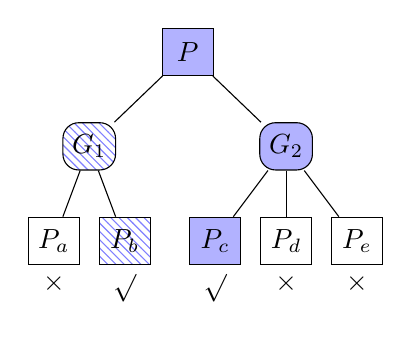
\begin{tikzpicture}[level distance=1.2cm]
\tikzstyle{succ}=[label=below:$\surd$]
\tikzstyle{fail}=[label=below:$\times$]
\tikzstyle{trace}=[solid,style=circle,fill=black!20,above left=0.15cm,scale=.7]

\tikzstyle{planbox}=[draw,minimum height=0.6cm,minimum width=0.65cm]
\tikzstyle{goalbox}=[draw,minimum height=0.6cm,minimum width=0.65cm,rounded corners=0.2cm]
\tikzstyle{planbox2}=[planbox,pattern=north west lines,pattern color=blue!50]
\tikzstyle{goalbox2}=[goalbox,pattern=north west lines,pattern color=blue!50]
\tikzstyle{goalbox3}=[goalbox,fill=blue!30]
\tikzstyle{planbox3}=[planbox,fill=blue!30]

\tikzstyle{level 1}=[sibling distance=2.5cm] 
\tikzstyle{level 2}=[sibling distance=0.9cm] 

\node[planbox3,solid] {$P$}
				child[solid] {node[goalbox2] {$G_{1}$}
					child {node[planbox,fail] {$P_{a}$}}
					child {node[planbox2,succ] {$P_{b}$}}
				}
				child[solid] {node[goalbox3] {$G_{2}$}
					child {node[planbox3,succ] {$P_{c}$}}
					child {node[planbox,fail] {$P_{d}$}}
					child {node[planbox,fail] {$P_{e}$}}
				}

;

\end{tikzpicture}

}}
\only<1>{Solution found at E=10 and \alert{full confidence at E=15}.}
\only<2->{
\resizebox{\textwidth}{!}{
%!TEX root = ../dsingh-phdtalk.tex
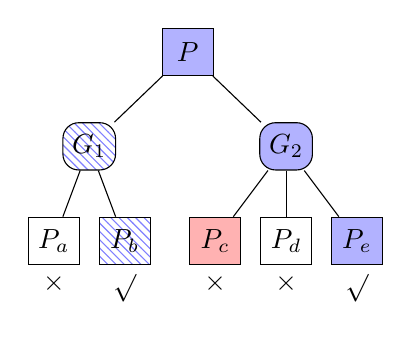
\begin{tikzpicture}[level distance=1.2cm]
\tikzstyle{succ}=[label=below:$\surd$]
\tikzstyle{fail}=[label=below:$\times$]
\tikzstyle{trace}=[solid,style=circle,fill=black!20,above left=0.15cm,scale=.7]

\tikzstyle{planbox}=[draw,minimum height=0.6cm,minimum width=0.65cm]
\tikzstyle{goalbox}=[draw,minimum height=0.6cm,minimum width=0.65cm,rounded corners=0.2cm]
\tikzstyle{planbox2}=[planbox,pattern=north west lines,pattern color=blue!50]
\tikzstyle{goalbox2}=[goalbox,pattern=north west lines,pattern color=blue!50]
\tikzstyle{goalbox3}=[goalbox,fill=blue!30]
\tikzstyle{planbox3}=[planbox,fill=blue!30]
\tikzstyle{planbox4}=[planbox,fill=red!30]

\tikzstyle{level 1}=[sibling distance=2.5cm] 
\tikzstyle{level 2}=[sibling distance=0.9cm] 

\node[planbox3,solid] {$P$}
				child[solid] {node[goalbox2] {$G_{1}$}
					child {node[planbox,fail] {$P_{a}$}}
					child {node[planbox2,succ] {$P_{b}$}}
				}
				child[solid] {node[goalbox3] {$G_{2}$}
					child {node[planbox4,fail] {$P_{c}$}}
					child {node[planbox,fail] {$P_{d}$}}
					child {node[planbox3,succ] {$P_{e}$}}
				}

;

\end{tikzpicture}

}}
\only<3>{
After E=15, $P_c$ starts to fail. The \alert{confidence drops}, promoting new exploration and re-learning.}
\end{overlayarea}
\end{column}
\begin{column}[l]{0.6\textwidth}
\begin{overlayarea}{\textwidth}{5cm} 
\only<1>{
\resizebox{\textwidth}{!}{
%!TEX root = ../dsingh-ijcai11-talk.tex
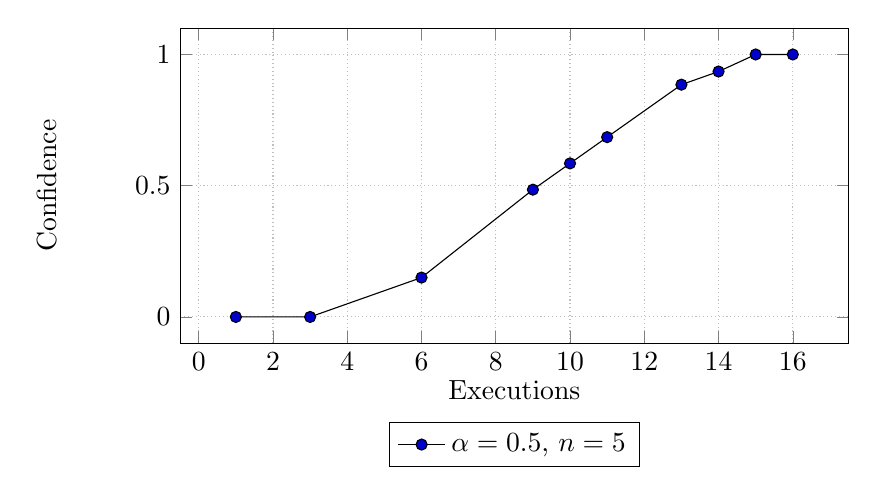
\begin{tikzpicture}

\begin{axis}[
width=0.7\columnwidth,height=4cm,scale only axis,
axis line style={-}, xtick style={-}, ytick style={-},
ymin=0,ymax=1, enlarge y limits=true,
xlabel=Executions,
ylabel=Confidence,
every axis y label/.style={at={(-0.2,0.5)},rotate=90,anchor=center}, 
every axis x label/.style={at={(0.5,-0.15)},anchor=center},
grid=both,grid style={-,style=densely dotted},
%legend style={at={(0.7,0.35)},anchor=north west},
legend style={at={(0.5,-0.25)}, anchor=north,legend columns=-1},
%cycle list name=black white,
] 

% alpha=0.5
\addplot+[black] coordinates { 
	(01,0.000) (03,0.000) (06,0.150) (09,0.485) (10,0.585) 
	(11,0.685) (13,0.885) (14,0.935) (15,1.000) (16,1.000) 
};
\addlegendentry{$\alpha=0.5$, $n=5$}

\end{axis} 
\end{tikzpicture} 

}}
\only<2>{~\\~\\\alert{What if the environment changes} after we have learnt the solution?\\~\\Say after execution $15$, plan $P_c$ no longer works for resolving goal $G_2$, but plan $P_e$ does.
}
\only<3>{
\resizebox{\textwidth}{!}{
%!TEX root = ../dsingh-ijcai11-talk.tex
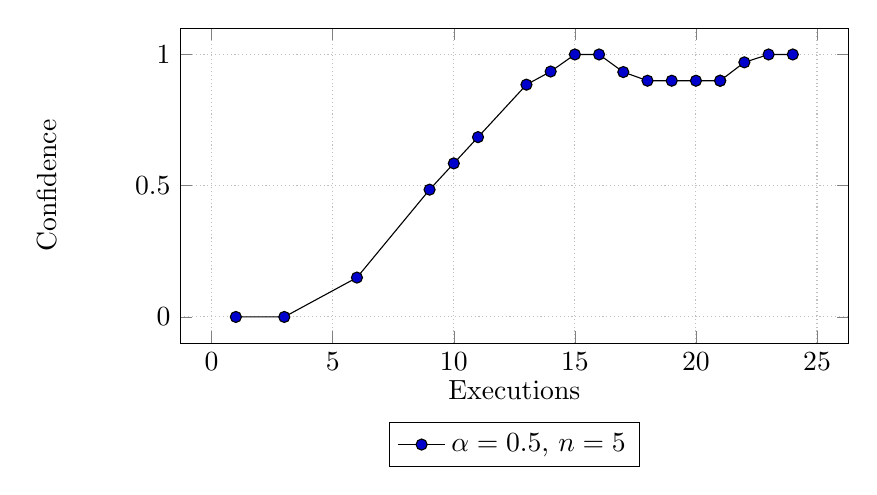
\begin{tikzpicture}

\begin{axis}[
width=0.7\columnwidth,height=4cm,scale only axis,
axis line style={-}, xtick style={-}, ytick style={-},
ymin=0,ymax=1, enlarge y limits=true,
xlabel=Executions,
ylabel=Confidence,
every axis y label/.style={at={(-0.2,0.5)},rotate=90,anchor=center}, 
every axis x label/.style={at={(0.5,-0.15)},anchor=center},
grid=both,grid style={-,style=densely dotted},
%legend style={at={(0.7,0.25)},anchor=north west},
legend style={at={(0.5,-0.25)}, anchor=north,legend columns=-1},
%cycle list name=black white,
] 

% alpha=0.5
\addplot+[black] coordinates { 
	(1,0.000) (3,0.000) (6,0.150) (9,0.485) (10,0.585) 
	(11,0.685) (13,0.885) (14,0.935) (15,1.000) (16,1.000) 
	(17,0.933) (18,0.900) (19,0.900) (20,0.900) (21,0.900) 
	(21,0.900) (22,0.970) (23,1.000) (24,1.000) 
};
\addlegendentry{$\alpha=0.5$, $n=5$}

\end{axis} 
\end{tikzpicture} 

}}
\end{overlayarea}
\end{column}
\end{columns}
\end{frame}

%----------------------------------------------------------------------------
%----------------------------------------------------------------------------
\section{Developing BDI Systems that Learn}

%----------------------------------------------------------------------------
%----------------------------------------------------------------------------
\subsection{Modular Battery System Controller}

%----------------------------------------------------------------------------
\begin{frame}{A Battery Storage Application}
\begin{columns}
\begin{column}[l]{0.6\textwidth}
%!TEX root = ../dsingh-ijcai11-talk.tex
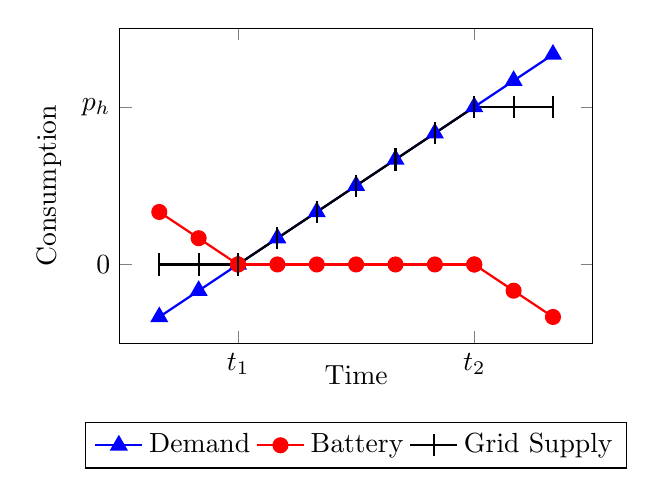
\begin{tikzpicture}

\begin{axis}[
width=6cm,height=4cm,scale only axis,
axis line style={-}, xtick style={-}, ytick style={-},
xlabel=Time,
ylabel=Consumption,
every axis y label/.style={at={(-0.15,0.5)},rotate=90,anchor=center}, 
every axis x label/.style={at={(0.5,-0.1)},anchor=center}, 
%grid=both, grid style={style=densely dotted},
xtick={2,8},
xticklabels={$t_1$,$t_2$},
ytick={0,6},
yticklabels={$0$,$p_h$},
legend style={at={(0.5,-0.25)}, anchor=north,legend columns=-1},
%legend style={at={(0.05,0.95)},anchor=north west}
] 

% Draw the Demand-Supply curve
\addplot[-,thick,color=blue,mark=triangle*,mark size=3.0] expression[domain=0:10,samples=11] {x-2};
\addlegendentry{Demand} 

% Draw the Battery curve
\addplot[-,thick,color=red,mark=*,mark size=2.5] expression[forget plot,domain=0:2,samples=3] {2-x}; 
\addplot[-,thick,color=red,mark=*,mark size=2.5] expression[forget plot,domain=2:8,samples=7] {0}; 
\addplot[-,thick,color=red,mark=*,mark size=2.5] expression[domain=8:10,samples=3] {8-x}; 
\addlegendentry{Battery} 

% Draw the Grid supply curve
\addplot[-,thick,mark=|,mark size=4] expression[forget plot,domain=0:2,samples=3] {0}; 
\addplot[-,thick,mark=|,mark size=4] expression[forget plot,domain=2:8,samples=7] {x-2}; 
\addplot[-,thick,mark=|,mark size=4] expression[domain=8:10,samples=3] {6}; 
\addlegendentry{Grid Supply} 
\end{axis} 
\end{tikzpicture} 

\end{column}
\begin{column}[r]{0.3\textwidth}
\begin{center}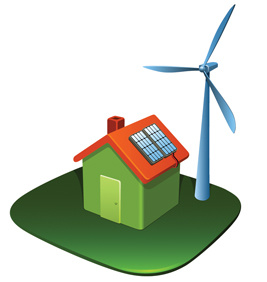
\includegraphics[scale=0.4]{figs/fig-storage-building}\end{center}
\end{column}
\end{columns}
Given net building demand, \alert{calculate an appropriate battery response} in order to maintain grid power consumption within range $[0,p_h]$.
\note{
Changing dynamics is when you learn something but the environment changes to that the learning is no longer optimal. Consider the example of a smart home..
}
\end{frame}

%----------------------------------------------------------------------------
\begin{frame}{Design: A Battery Storage Application}
\begin{center}
\resizebox{0.8\textwidth}{!}{
%!TEX root = ../dsingh-pgconf10.tex
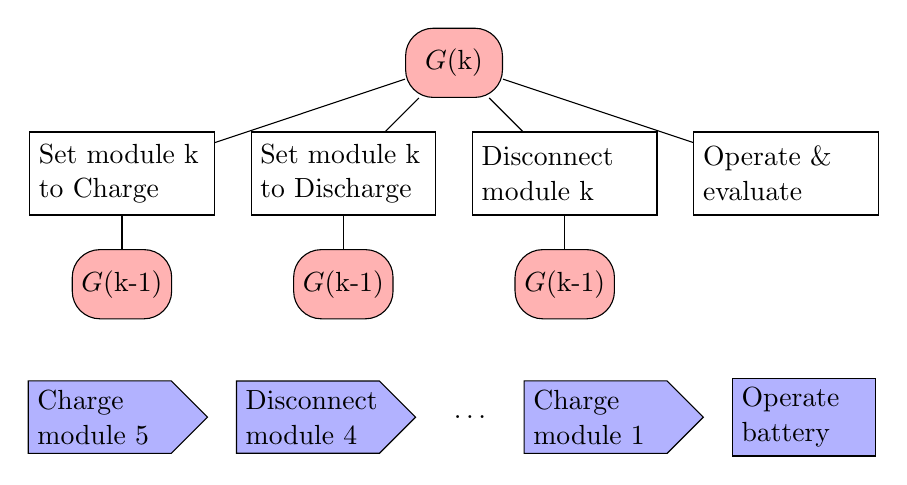
\begin{tikzpicture} [start chain,level distance=4.0em,node distance=1.0em]
\tikzstyle{planbox}=[draw,text width=6.0em,minimum height=3.0em]
\tikzstyle{goalbox}=[draw,rounded corners=1.0em,minimum height=2.5em,minimum width=3.5em,fill=red!30]

\tikzstyle{level 1}=[sibling distance=8.0em] 

\tikzstyle{chainbox}=[{
draw,
fill=blue!30,
on chain,
minimum height=2.5em,minimum width=5.0em,text width=4.5em,
}]
\tikzstyle{chainbox2}=[chainbox,shape=signal,signal to=east]


\node[goalbox,solid] at (0,0) {$G($k$)$}
	child {node[planbox] {Set module k to \alert{Charge}}
		child {node[goalbox] {$G($k-1$)$}}
	}
	child {node[planbox] {Set module k to \alert{Discharge}}
		child {node[goalbox] {$G($k-1$)$}}
	}
	child {node[planbox]  {\alert{Disconnect} module k}
		child {node[goalbox] {$G($k-1$)$}}
	}
	child {node[planbox]  {\alert{Operate} \& evaluate}}
;


\node[chainbox2]  at (-4.5,-4.5) {Charge module 5};
\node[chainbox2]  {Disconnect\\module 4};
\node[on chain] (C){$\ldots$};
\node[chainbox2]   (D) {Charge module 1};
\node[chainbox]    (E) {Operate\\battery};

\end{tikzpicture}



}
\end{center}
Aim: Learn appropriate plan selection to achieve a desired \alert{battery response rate}, given the current battery state. \example{State space for a battery with five modules is $\approx$13 million.}
\end{frame}

%----------------------------------------------------------------------------
\begin{frame}[allowframebreaks]{Experiment: Capacity Deterioration}

\begin{center}
%!TEX root = ../dsingh-ijcai11-talk.tex
\begin{tikzpicture}

\begin{axis}[
width=0.7\columnwidth,height=5cm,scale only axis,
axis line style={-}, xtick style={-}, ytick style={-},
xlabel=Episodes,
ylabel=Success,
every axis y label/.style={at={(-0.15,0.5)},rotate=90,anchor=center}, 
every axis x label/.style={at={(0.5,-0.15)},anchor=center},
grid=both,grid style={-,style=densely dotted},
legend style={at={(0.5,0.25)},anchor=north west},
scaled x ticks = false,
xtick={0,5e3,10e3,15e3,20e3,25e3,30e3,35e3,40e3},
xticklabels={$0$,$5\kilo$,$10\kilo$,$15\kilo$,$20\kilo$,$25\kilo$,$30\kilo$,$35\kilo$,$40\kilo$}
] 

\addplot[-,red,thick] file {./data/storage1b.CF.tikzdata};
%\addlegendentry{Data} 

\end{axis} 
\end{tikzpicture} 


Recovery from \alert{deterioration in module capacities} at $5\kilo$ episodes.
\end{center}
\end{frame}

%----------------------------------------------------------------------------
\begin{frame}[allowframebreaks]{Experiment: Partial Failure with Restoration}
\begin{center}
%!TEX root = ../dsingh-ijcai11-talk.tex
\begin{tikzpicture}

\begin{axis}[
width=0.7\columnwidth,height=5cm,scale only axis,
axis line style={-}, xtick style={-}, ytick style={-},
%xlabel=Episodes,
%ylabel=Success,
every axis y label/.style={-,at={(-0.12,0.5)},rotate=90,anchor=center}, 
%every axis x label/.style={at={(0.5,-0.15)},anchor=center},
grid=both,grid style={-,style=densely dotted},
legend style={at={(0.5,0.25)},anchor=north west},
scaled x ticks = false,
xtick={0,5e3,10e3,15e3,20e3,25e3,30e3,35e3,40e3},
xticklabels={$0$,$5\kilo$,$10\kilo$,$15\kilo$,$20\kilo$,$25\kilo$,$30\kilo$,$35\kilo$,$40\kilo$}
] 

\addplot[-,red,thick] file {./data/storage2b.CF.tikzdata};
%\addlegendentry{Data} 

\end{axis} 
\end{tikzpicture} 


Recovery from \alert{temporary module failures} during $[0,20\kilo]$, $[20\kilo,40\kilo]$ episodes.
\end{center}
\end{frame}

%----------------------------------------------------------------------------
\begin{frame}[allowframebreaks]{Experiment: Complete Failure with Restoration}
\begin{center}
%!TEX root = ../dsingh-ijcai11-talk.tex
\begin{tikzpicture}

\begin{axis}[
width=0.7\columnwidth,height=5cm,scale only axis,
axis line style={-}, xtick style={-}, ytick style={-},
%xlabel=Episodes,
%ylabel=Success,
every axis y label/.style={-,at={(-0.12,0.5)},rotate=90,anchor=center}, 
%every axis x label/.style={at={(0.5,-0.15)},anchor=center},
grid=both,grid style={-,style=densely dotted},
legend style={at={(0.5,0.25)},anchor=north west},
scaled x ticks = false,
xtick={0,5e3,10e3,15e3,20e3,25e3,30e3,35e3,40e3},
xticklabels={$0$,$5\kilo$,$10\kilo$,$15\kilo$,$20\kilo$,$25\kilo$,$30\kilo$,$35\kilo$,$40\kilo$}
] 

\addplot[-,red,thick] file {./data/storage3mb.CF.tikzdata};
%\addlegendentry{Data} 

\end{axis} 
\end{tikzpicture} 


Recovery from \alert{complete system failure} during $[0,5\kilo]$ episodes.
\end{center}
\end{frame}


%----------------------------------------------------------------------------
%----------------------------------------------------------------------------
\section{Conclusions and Future Work}

%----------------------------------------------------------------------------
\begin{frame}{Limitations and Future Work}
\begin{itemize}
\item<+-> We cannot account for \alert{inter-dependence between subgoals} of a higher-level plan.\\~\\
\item<+-> \alert{Maintaining full training data is not practical}. It becomes obsolete when the environment changes. \example{We tried an arbitrary scheme to filter ``old'' data in the battery agent and reduced the data set by $75\%$ with no loss in performance.}\\~\\
\item<+-> Onus is on the designer to select appropriate state representation and learning parameters. \example{Some of this could be automatically extracted from the BDI program.}
\end{itemize}
\end{frame}

%----------------------------------------------------------------------------
\begin{frame}[<+->]{Summary}
\action{}
\begin{itemize}
\item Learning BDI plan selection is desirable when plan applicability cannot be easily programmed or when the \alert{environment changes over time}.\\~\\
\item We present a \alert{learning framework} for additionally determining a plan's applicability conditions using decision trees. Plans are selected \alert{probabilistically} based on their predicted likelihood of success and our perceived \alert{confidence} in the learning.\\~\\
\item We evaluate the framework empirically in a storage domain where a battery controller must continually adapt to \alert{changes that cause previous solutions to become ineffective}.
\end{itemize}
\end{frame}

%----------------------------------------------------------------------------
%----------------------------------------------------------------------------
\setcounter{finalframe}{\value{framenumber}}
\appendix 

\begin{frame}{References}
\setcounter{framenumber}{\value{finalframe}}
  \begin{thebibliography}{10}
  \beamertemplatearticlebibitems
  \bibitem{singh10:extending}
	D.~Singh, S.~Sardina, L.~Padgham.
	\newblock Extending BDI plan selection to incorporate learning from experience.
	\newblock {\em Journal of Robotics and Autonomous Systems (RAS)}, 2010.
  \bibitem{singh10:learning}
	D.~Singh, S.~Sardina, L.~Padgham, and S.~Airiau.
	\newblock Learning context conditions for BDI plan selection.
	\newblock {\em Proceedings of Autonomous Agents and Multi-Agent Systems (AAMAS)}, 2010.
  \bibitem{airiau09:enhancing}
	S.~Airiau, L.~Padgham, S.~Sardina, and S.~Sen.
	\newblock Enhancing adaptation in {BDI} agents using learning techniques.
	\newblock {\em International Journal of Agent Technologies and Systems (IJATS)}, 2009.\\~\\
  \end{thebibliography}

\begin{block}{}\centering{\alert{Poster today in Rooms 133--134 at 16:40--17:20}}\end{block}

\end{frame}


%----------------------------------------------------------------------------
%----------------------------------------------------------------------------
%----------------------------------------------------------------------------
%----------------------------------------------------------------------------
%----------------------------------------------------------------------------
%----------------------------------------------------------------------------
%%%

\end{document}
